% This is a LaTeX thesis template for Monash University.
% to be used with Rmarkdown
% This template was produced by Rob Hyndman
% Version: 6 September 2016

\documentclass{monashthesis}

%%%%%%%%%%%%%%%%%%%%%%%%%%%%%%%%%%%%%%%%%%%%%%%%%%%%%%%%%%%%%%%
% Add any LaTeX packages and other preamble here if required
%%%%%%%%%%%%%%%%%%%%%%%%%%%%%%%%%%%%%%%%%%%%%%%%%%%%%%%%%%%%%%%

\author{Zhixiang Yang}
\title{Disaggregated Sectoral Employment Dynamics in Australia}
\studentid{30306396}
\def\degreetitle{Bachelor of Commerce (Honours)}
% Add subject and keywords below
\hypersetup{
     %pdfsubject={The Subject},
     %pdfkeywords={Some Keywords},
     pdfauthor={Zhixiang Yang},
     pdftitle={Disaggregated Sectoral Employment Dynamics in Australia},
     pdfproducer={Bookdown with LaTeX}
}


\bibliography{thesisrefs}

\begin{document}

\pagenumbering{roman}

\titlepage

{\setstretch{1.2}\sf\tighttoc\doublespacing}

\clearpage\pagenumbering{arabic}\setcounter{page}{0}

\hypertarget{acknowledgement}{%
\chapter*{Acknowledgement}\label{acknowledgement}}
\addcontentsline{toc}{chapter}{Acknowledgement}

I would like to express gratitude to my supervisor Professor Farshid Vahid and my coordinatior Professor Heather Anderson for their selfless support and devoted care along the way.

\hypertarget{declaration}{%
\chapter*{Declaration}\label{declaration}}
\addcontentsline{toc}{chapter}{Declaration}

I declare that this thesis contains no material which has been submitted in any form for the award of any other degree or diploma in any university or equivalent institution, and that, to the best of my knowledge and belief, this thesis contains no material previously published or written by another person, except where due reference is made in the text of the thesis.

\vspace{12pt}

-- Signature: \underline{\emph{\textbf{Elvis Zhixiang Yang}}}

\hypertarget{abstract}{%
\chapter*{Abstract}\label{abstract}}
\addcontentsline{toc}{chapter}{Abstract}

I develop a multivariate time series model of employment in Australia at a disaggregated level with 87 sectors in total. I use this model to determine the long run employment spillovers to the total employment at this level. Our findings is that \ldots{}

Moreover, I provide an interactive shiny app that will give an intuitive visualization of these changes. At the stage of recovering from COVID-19, it will provide more useful information for policymakers on recovering total employment rate more effectively.

\hypertarget{the-australian-covid-19-pandemic-background}{%
\chapter{The Australian COVID-19 Pandemic Background}\label{the-australian-covid-19-pandemic-background}}

The COVID-19 pandemic has had a massive effect on economies around the world. Across different countries, millions of workers were furloughed or even lost their jobs as businesses struggled to survive \autocite{ny2020}. The same situation happened in Australia, due to more restrictions, many businesses closed their doors, while employees were working with less hours or being dismissed by companies. As a result of the continuous ``lockdown'' periods in 2020, estimates made by the Australian Bureau of Statistics \autocite{ABS2021} concluded that 72\% of businesses generated less revenue and the underemployment rate hit a historical high of 13.8\% by the end of April, 2020, only one month after the COVID-19 outbreak.

Our research is motivated by the lack of quantitative research on the employment of two-digit disaggregated industry sectors in Australia, as many studies have focused on the aggregated employment rate. A general problem of aggregated research is the loss of hierarchical information, which may result in a biased conclusion or ``an illusion of employment prosperity''. Thus, a quantitative analysis of the sectoral employment will ameliorate this problem, giving us a better scope to evaluate the impacts of COVID-19 in Australia.

\hypertarget{research-aim-and-questions}{%
\section{Research Aim and questions}\label{research-aim-and-questions}}

This research will extend \textcite{anderson2020} by using data on 87 two-digit industry sectors instead of 19 sectors that they used. I will develop a model for the two-digit sectors to evaluate the long run effect and the COVID-19 post-impacts. I will also provide a counterfactual analysis based on the assumption ``if there is no pandemic''. The two-digit sectoral data will provide us with more information, which will assist in getting a better understanding of employment dynamics in Australia.

The overall research aim is to provide estimates of two-digit sectoral employment based on historical data. Specifically, my goals are:

\begin{enumerate}
\def\labelenumi{\arabic{enumi}.}
\item
  To construct a time series model of employment in 87 two-digit sectors of the Australian economy.
\item
  To use this model to conduct a counterfactual analysis.
\item
  To use this model to determine which two-digit sectors have the highest impact (or positive spillover) on employment growth in the long run.
\end{enumerate}

\hypertarget{thesis-structure}{%
\section{Thesis Structure}\label{thesis-structure}}

This thesis focus on analyzing Australian Employment at a disaggregated level, then estimate the long run effects of the COVID-19 to sectoral employment rate in Australia. The remainder of the thesis is structured as follows. In chapter 2, we review the existing literature in the relevant fields. In chapter 3, we will provide exploratory data analysis and data resources.

\clearpage

\hypertarget{review-of-literature}{%
\chapter{Review of literature}\label{review-of-literature}}

Our review of literature mainly focuses on two areas:

\begin{enumerate}
\def\labelenumi{\arabic{enumi}.}
\item
  The COVID-19 sectoral impacts and modelling of the economy.
\item
  Modelling of large numbers of time series.
\end{enumerate}

\hypertarget{sectoral-impact-of-covid-19.}{%
\section{Sectoral Impact of COVID-19.}\label{sectoral-impact-of-covid-19.}}

Most existing studies have focused on the evaluation of the impacts of COVID-19 on broad sectors of large economies such as the US and Europe. \textcite{ludvigson2020covid} developed a disaster series to translate the macroeconomic impact of costly and deadly disasters in recent US history and model them as sectoral shocks to predict COVID-19. They concluded that the shock would lead to a cumulative loss of 20\% in industrial production, 39\% in public services and also reduce the US GDP by 12.75 per cent at the end of 2020. \textcite{gregory2020pandemic} conducted simulations under different scenarios via a search theoretic model using US data and found the recovery in the US is L-shaped, with employment remaining lower than pre-covid for a long period. They also extended their studies at a disaggregated level of 20 sectors, showing that ``arts and entertainment'' and ``accommodation and food services'' sectors would have the biggest shock during the pandemic.

In Australia, \textcite{anderson2020} developed a multivariate time series model for 19 main sectors in Australia (as a small open economy) using a Bayesian VARX model. Their research concluded that ``Manufacturing'' and ``Construction'' have the highest positive spillovers for the aggregate economy. Meanwhile, they also applied a ``conditional forecasting'' method proposed by \textcite{waggoner1999} to simulate different scenarios for the pandemic in Australia. However, their research does not use a finely disaggregated level in Australia (two-digit subsectors of main sectors), which can be extremely useful in macroeconomic analysis.

\hypertarget{modelling}{%
\section{Modelling}\label{modelling}}

\hypertarget{baysian-var}{%
\subsection{Baysian VAR}\label{baysian-var}}

The Bayesian Vector Autoregression model (BVAR) is commonly used in the literature for multivariate data \autocites[e.g.][]{anderson2020,litterman1986,banbura2010large}. The BVAR model is attractive because it allows us to estimate a large number of parameters, when the sample size is not large, in a statistically coherent way.\autocite{litterman1986,wozniak2016bayesian}.

In order to utilize the Bayesian VAR estimators \textcite{litterman1979} proposed the Minnesota Prior, which decreases the weight of the lagged variable with the lag length. The prior mean on the first own lag is set to unity and the rest are set to zero so that (a) the most recent lag should provide more information than distant lags; and (b) own lags should explain more than the lags of other variables.

\hypertarget{improvement-of-bvar}{%
\subsection{Improvement of BVAR}\label{improvement-of-bvar}}

The literature suggests that a significant improvement can be made in large BVAR dynamic models by imposing a stronger shrinkage parameter \autocite{banbura2010large,litterman1986}. \textcite{robertson1999vector} and \textcite{kadiyala1997} proposed a Normal-inverse-Wishart prior which retains the principal of Minnesota prior. Meanwhile, \textcite{banbura2010large} suggested an easier way to apply the Minnesota prior via adding dummy observations into the BVAR system.

\clearpage

\hypertarget{data-collection-and-exploratory-analysis}{%
\chapter{Data collection and exploratory analysis}\label{data-collection-and-exploratory-analysis}}

\hypertarget{data-introduction-and-wrangling}{%
\section{Data Introduction and wrangling}\label{data-introduction-and-wrangling}}

The data I use in this thesis come from the Australia Bureau of Statistics (ABS), involving 87 industry sub-division of main jobs. The ABS records the employment (measured in \(thousands\)) from \(1984:Q4\) to \(2021:Q4\) with a structure provided via Figure \ref{fig:anzsic}.

Although seasonally adjusted data is available in \autocite{ABS2022}, the method of seasonal adjustment used by ABS is unknown. Therefore, I choose to work with the original data to capture any possible changes in seasonal patterns instead of the seasonally adjusted data provided by Australian Bureau of Statistics.

Since the original data from ABS is not tidy. In this thesis, I use the Excel to extract both the employment for both two-digit disaggregated level and the total employment. Then, I take the following modifications to deal with zeros, meanwhile, keeping the data structure coherent.

\begin{itemize}
\item
  Merge the two-digit subsector \emph{57- Internet Publishing and Boardcasting} and \emph{54- Publishing(except internet)} to be come \emph{54 Publishing and boadcasting}.
\item
  Merge the \emph{96 Private Households Employing Staff and Undifferentiated Goodsand Service Producing Activities of Households for Own Use} and \emph{95 Personal and Other Services} to become \emph{95 Personal and other services (include activities for own use)}.
\end{itemize}

Without any zeros, a log transformation can be applied to interprete the percentage change of the employment. The VAR model decided to fit the data requires stationary. As a result, I will further apply a seasonal difference to eliminate the seasonality (i.e.~nonstationarity).

\hypertarget{preliminary-exploratory-data-analysis}{%
\section{Preliminary Exploratory Data Analysis}\label{preliminary-exploratory-data-analysis}}

Figure \ref{fig:19} illustrates the changes in the raw data for 19 main sectors in Australia during the pandemic. Due to the closedown of businesses and travel bans on 2020:Q2, we can observe that the total employment number dropped substantially (from around 13,200,000 to 12,200,000 on \(2020:Q2\)). Most industries behaved similarly with significant changes shown in Figure \ref{fig:19} . Comparing with the previous data of these industries,'' Accommodation \& Food'', ``Media \& telecom'' and Administrative industries have experienced a severe loss of employment and have not fully recovered to the pre-covid level. However, some industries like ``Financial'' and ``Electricity \& Gas'' showed a continuously increasing trend as before.

Nevertheless, there is a drawback of considering the 19 board sectors only; because the two-digit subsectoral dynamics of these sectors may not be homogeneous with their aggregated sectoral changes. For example, when observing the aggregated performance of the ``Manufacturing'' and ``Mining'' sectors from the 19 sectoral level (see Figure \ref{fig:a19}), we may believe that their corresponding subsectors should illustrate the same pattern. However, the reality is that while there is a decreasing trend in the ``Manufacturing'' sector or an increasing trend in the ``Mining'' sector, some of their two-digit subsectors are performed differently (see Figure \ref{fig:a87}). This means that not all two-digit subsectors follow the same pattern with the aggregated sectoral level.

Table \ref{tab:comp} shows the top five and bottom five two-digit subsectors in terms of their employment growth during the pandemic. From \ref{tab:comp} we can conclude that the ``Forestry and Logging'' experienced a severe shock after the lockdown happened on 2020:Q2, followed by ``Private Households Employing Staff'' and ``Library and Other Information Services''. Figure \ref{fig:87} demonstrates the performance of each industry at a more disaggregated two-digit subsectoral level, we can observe that many two-digit subsectors have also shown huge decreases in employment in 2020:Q2.

\begin{table}
\begin{center}
\begin{tabular}{ccc}
\hline
Date     & Sector                                        & Percentage Changes \\
\hline
2020:Q2  & 27 Gas Supply                                 & 50.48\%                                \\
2020: Q2 & 57 Internet Publishing and Broadcasting       & 44.44\%                                \\
2020: Q2 & 56 Broadcasting                               & 41.43\%                                \\
2020: Q2 & 26 Electricity Supply                         & 36.34\%                                \\
2020: Q2 & 20 Non-Metallic Mineral Product Manufacturing & 32.37\% 
                 \\
                 \\
                 \hline
Date     &  Sectors                                      &Percentage Changes\\
                 \hline
2020: Q2 & 03 Forestry and Logging                   &-55.88\%  
                 \\
2020: Q2 & 96 Private Households Employing Staff     & -49.09\% 
                 \\
2020: Q2 & 60 Library and Other Information Services & -46.60\% 
                 \\
2020: Q2 & 02 Aquaculture                                & -44.58\%  
                 \\
2020: Q2 & 91 Sports and Recreation Activities           & -43.71\%
\end{tabular}
\end{center}
\caption{The highest and lowest five two-digit subsectors' employment percentage change for 2020:Q1 to 2020:Q2 }
\label{tab:comp}
\end{table}

\hypertarget{methdology}{%
\chapter{Methdology}\label{methdology}}

\hypertarget{proposed-model}{%
\section{Proposed Model}\label{proposed-model}}

I plan to use a Bayesian VARX model based on a method proposed by \textcite{anderson2020}. In the model, each sector is affected by the lags of sectoral growth and a lag of the total employment growth. The lag of aggregate employment growth acts as an economy-wide factor which will affect each sector.

Under the assumption that the structure of the Australian economy will not change during COVID-19, we suggest the BVAR model as

\[
\begin{aligned}
\textbf{y}_t=\textbf{c}+\textbf{A}_1 \textbf{y}_{t-1}+\textbf{A}_2\textbf{y}_{t-2}+\textbf{A}_3\textbf{y}_{t-3}+\textbf{A}_4\textbf{y}_{t-4}+\boldsymbol{\Gamma}\textbf{x}_{t-1}+\bf{u}_t
\end{aligned}
\]

where \(\bf{y}_t\) is an \(87\times1\) vector of two-digit subsectoral employment growth rate at time \(t\) and \(\bf{x}_{t-1}\) is the \(4\times1\) vector of 4 lags of the growth rate of aggregate employment (this vector of variables are predetermined at time \(t\)), \(\textbf{c}\) is a vector of constants, \(\bf{A}_{1,2,3,4}\) are \(87\times87\) parameter matrices. \(\boldsymbol{\Gamma}\) is a \(87\times4\) matrix and \(\bf{u}_t\) is a vector of reduced form errors with the mean equals to zero and independent variance \(\bf{u}_t \sim (0,\boldsymbol{\Sigma})\). (see Appendix)

\hypertarget{prior-and-shrinkage}{%
\section{Prior and shrinkage}\label{prior-and-shrinkage}}

Bayesian VAR helps to overcome the curse of high dimensionality via the imposition of prior beliefs on the parameters \autocite{banbura2010large}. I will estimate the VARX using Bayesian methods by specifying a Minnesota prior \autocites[e.g.][]{anderson2020,litterman1986,robertson1999vector}. In order to set up the Minnesota prior in our BVAR model, \textcite{banbura2010large} suggests a Minnesota-type prior that applies shrinkage to the VAR slope coefficients as follows:

\[
\begin{aligned}\label{eq:1}
&E[a_{i}^{jk}] = E[\gamma_{i}^j]=0\\
\\
&Var[a_i^{jk}]= 
\begin{cases}
\frac{\lambda^2}{i^2},&j=k\\
\frac{\lambda^2}{i^2}\frac{\sigma^2_{j}}{\sigma^2_k},& otherwise
\end{cases}\\
\\
&Var[\gamma_i^{j}]=\frac{\lambda^2}{i^2}\frac{\sigma^2_{j}}{\sigma^2_e}
\end{aligned}
\]
where the degree of shrinkage is governed by \(\lambda\), \(\frac{1}{i^2}\) to down-weight more distant lags and the \(\frac{\sigma_j^2}{\sigma_k^2}\) adjusts for different scale of the data. \(\sigma^2_e\) is the variance after fitting an AR model on total employment growth.

\textcite{banbura2010large} also suggested that a natural conjugate Normal-Inverse-Wishart which retains the principle of Minnesota prior will help in adding Minnesota prior to the Bayesian VAR system. Its posterior moments can be calculated either analytically or through adding the dummy observations. I will use dummy observations to estimate the BVAR \autocite{banbura2010large}. More details are provided in the Appendix.

\newpage

\hypertarget{shrinkage-selection-in-bayesian-var}{%
\section{Shrinkage selection in Bayesian VAR}\label{shrinkage-selection-in-bayesian-var}}

Specifically, the Minnesota type prior have the following beliefs about the variances:

\[
\begin{aligned}
&Var[a_i^{jk}]= 
\begin{cases}
\frac{\lambda^2}{i^2},&j=k\\
\frac{\lambda^2}{i^2}\frac{\sigma^2_{j}}{\sigma^2_k},& otherwise
\end{cases}\cdots(4.3.1)\\
\\
&Var[\gamma_i^{j}]=\frac{\lambda^2}{i^2}\frac{\sigma^2_{j}}{\sigma^2_e}\cdots(4.3.2)
\end{aligned}
\]

where \(\lambda\) is a hyperparemeter here we need to specify based on how far we will shrink the estimator and \(\frac{\sigma^2_{j}}{\sigma^2_k}\) adjusts for the different scale of the data. To effectively scale the estimator on total employment growth \(\gamma\), I will fit an AR(4) to on the total employment growth \autocite{anderson2020}.

In equation \(4.3.1\), we can see as \(i\) (number of estimators) increases, the \(Var[a_i^{jk}]\) will then decrease in both cases, which preserved the structure of Minnesota Prior to weight down more distant lags.

In Minnesota prior described above, the hyperparameter \(\lambda\) controls the overall tightness (variance) of the prior distribution \autocite{banbura2010}. If \(\lambda=0\), we can see that the prior have no variance, which means the posterior equals the prior and the data have no influence on the estimates. On the contrary, if \(\lambda=\infty\), the posterior expectations will be same as ordinary least squares (OLS) estimates. Therefore, a small \(\lambda\) will shrink the posterior mean towards the zero and benefits .

Admittedly, the selection of shrinkage hyperparameter \(\lambda\) is important in improving forecast accuracy. For example, \textcite{banbura2010large} point out that a gain in efficiency could be made by applying an Bayesian shrinkage in estimating large multivariate VAR models. Moreover, they also conclude that large vector autoregressions (VARs) with shrinkage are credible to conduct structural analysis. Nonetheless, the main problem that encountered is to set an appropriate value for \(\lambda\) as models become larger (i.e.~how far it will shrink the estimators).

From the above equation, we can see a small shrinkage parameter \(\lambda\) will tighten the distribution of prior, and vice versa. Based on applied experiences, Litterman constructed a 40-variable model and concluded that the shrinkage estimate \(\lambda=0.2\) is indeed sufficient to deal with many empirical cases \autocite{litterman1986}. At the same time, I should also avoid over-fitting when preserving the most important information from the data. That is, the data size is also an essential basis to be considered when deciding the degree of shrinkage\autocite{banbura2010large}. Unlike the one-digit level (19 sectors) did by \textcite{anderson2020}, the two-digit level (87 sectors) employment in Australia is more complex and have more variables. Thus, a new shrinkage parameter \(\lambda\) should be specified particularly for this case.

In this section, I will evaluate the efficient shrinkage estimator \(\lambda\) with a more sophisticated version of training/test algorithm, called time series cross-validation. The time-series cross validation is an automated program based on a rolling forecasting origin, which measure the performance of a model in a statistical way while avoiding over-fitting the data. Here, the data is split into training/test with a minimum training set of length \(n=20\). Then, the program will increasing the size of successive training set by iteration step \(hor=1\) and accumulate the error for each step. After that, it will calculate the mean of accumulated error, which will be the training results (see Figure \ref{fig:tscv}).

\graphicspath{ {/Users/elvisyang/Desktop/hon_proj/Disaggregated_Employment/Honours_thesis/figures} }

\begin{figure}[t]
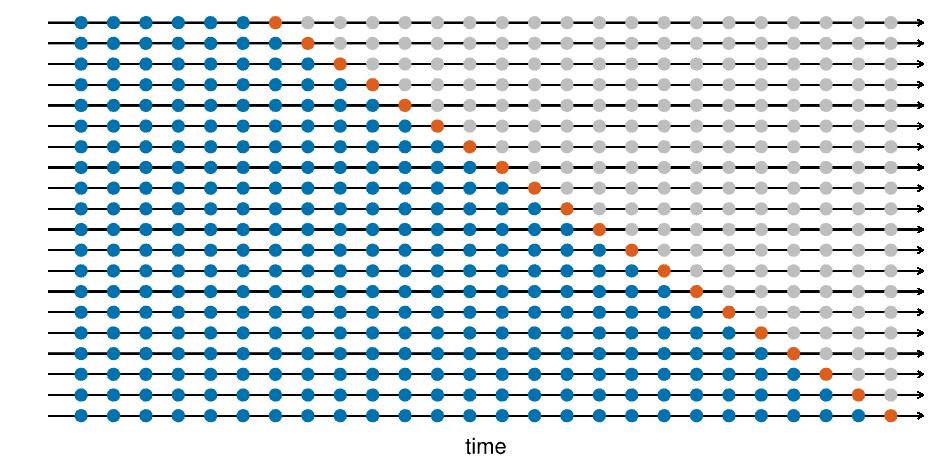
\includegraphics[scale=0.5]{tscv}
\centering
\caption{Time series cross validation with Blue area is training set and Orange is test set, with iteration step = 1 (Source https://otexts.com/fpp3/tscv.html)}
\label{fig:tscv}
\end{figure}

Apart from this, we will use several famous error measures to select an appropriate shrinkage parameter \(\lambda\):

\emph{Scale-dependent error}

\begin{itemize}
\item
  Mean absolute error: \(MAE = mean(|e_t|)\)
\item
  Root mean squared error: RMSE = \(\sqrt{mean(e_t^2)}\)
\end{itemize}

In the real world, MAE and RMSE are commonly used, but only when data all have the same units. They are easy to understand and calculate, which makes them popular to compare forecast accuracy. Nevertheless, they have a significant drawback, which is not unit-free.

\emph{Percentage error :}

\begin{itemize}
\tightlist
\item
  Mean absolute percentage error: \(MAPE = mean(|\frac{e_t}{y_t}|)\)
\end{itemize}

The percentage error (i.e.~MAPE) has the advantage of being unit-free. However, it will become unreliable when the data have zeros or extreme values (i.e.~very close to zero). As a result, I will use it only as a reference in this literature.

\emph{Scale-independent error:}

\begin{itemize}
\item
  MASE: \(MASE = mean(|q_j|)\)
\item
  RMSSE = \(RMSSE=\sqrt{mean(q_j^2)}\)
\end{itemize}

where

\(q_j^2=\frac{e_j}{\frac{1}{T-m}\Sigma^T_{t=m+1}|y_t-y_{t-m}|}\) and \(m\) is the seasonality. In this case, we set \(m=1\) after a seasonal difference and logarithm transformation, which is used for stationary (i.e.~non-seasonal) data.

MASE and RMSSE are useful when comparing forecast accuracy across data with different units \autocite{hyndman2006}. Both of them are scaled based on the same measure but from a simple forecast method. Since the employment data have a strong seasonality, the scaled error is defined using random walk with drift forecasts.

\vspace{24pt}

Table \ref{testres} demostrates the training results for \(\lambda\) with the following values \(0.3,0.2,0.19 \cdots 0.14\) and \(0.1\) after using the time series cross validation algorithm

\begin{table}[h]
\begin{center}
\begin{tabular}{|p{2cm}|p{2cm}|p{2cm}|p{2cm}|p{2cm}|p{2cm}|}
\hline\hline
\multicolumn{6}{|c|}{Training results using time-series cross validation}\\
\hline
\multicolumn{6}{|c|}{initial training (n = 20) ; iteration step (hor = 1)}\\
\hline\hline
 $\lambda$    & MAE         & MAPE    & MASE   & RMSE    & RMSSE  \\
\hline\hline
0.3  & 1.0832 e+03 & 14.5901 & 0.1465 & 32.5049 & 0.3778 \\
0.21 & 1.0738 e+03 & 14.1178 & 0.1457 & 32.3324 & 0.3765 \\
0.2  & 1.0727 e+03 & 14.0599 & 0.1457 & 32.3137 & 0.3764 \\
0.19 & 1.0715 e+03 & 14.0000 & 0.1455 & 32.2937 & 0.3762 \\
0.18 & 1.0701 e+03 & 13.9371 & 0.1454 & 32.2713 & 0.3760 \\
0.17 & 1.0685 e+03 & 13.8707 & 0.1453 & 32.2461 & 0.3758 \\
0.16 & 1.0668 e+03 & 13.8006 & 0.1451 & 32.2180 & 0.3756 \\
0.15 & 1.0648 e+03 & 13.7253 & 0.1449 & 32.1870 & 0.3753 \\
0.14 & 1.0626 e+03 & 13.6450 & 0.1446 & 32.1531 & 0.3750 \\
0.1  & 1.0512 e+03 & 13.2350 & 0.1433 & 31.9753 & 0.37333\\
\hline\hline
\end{tabular}
\end{center}
\caption{Forecast error for different hyperparameter $\lambda$}
\label{testres}
\end{table}

To sum up, We prefer the value of \(\lambda\) that has the lowest error measures. From table \ref{testres}, all the errors are decreasing as the shrinkage estimator becomes stronger (i.e.~the value of lambda becomes smaller). In this case, the shrinkage hyperparameter \(\lambda=0.1\) outperforms other values in our training steps. Therefore, the optimal value of the shrinkage parameter \(lambda\) for the Minnesota prior in our Bayesian VAR model is \(\lambda=0.1\).

\hypertarget{sectoral-employment-multiplier-analysis}{%
\section{Sectoral Employment Multiplier Analysis}\label{sectoral-employment-multiplier-analysis}}

I will also conduct a two-digit subsectoral employment multiplier analysis based on the estimated BVAR model and the 87 two-digit subsectoral data.

At each time period, we have :

\[
GR_T=\sum_{j=1}^{87} w_j\times {GR}_j
\]

where \(w_j\) is the share of employment of two-digit subsector \(j\) in the total employment, \(GR_T\) is the growth rate in total employment and \(GR_j\) is the growth rate in employment of two-digit subsector \(j\).

Due to the interconnection of macroeconomic two-digit subsectors, when a two-digit subsector \(j\) has an increase in employment, in the long run, it may have spillover effect onto other two-digit subsectors, especially those that have high connections with the two-digit subsector \(j\) (\textcite{anderson2020}).

If this long-run effect is larger than the immediate effect, then this two-digit subsector will have positive spillover effect on total employment, and \emph{vice versa}. I will use the interconnection of BVAR parameters to study two-digit subsectors which have strong positive spillovers for the total employment. Then, if the government makes policies to stimulate these two-digit subsectors, the total employment will recover more effectively.

\newpage

\hypertarget{timeline-for-honours-2022}{%
\chapter{Timeline for Honours 2022}\label{timeline-for-honours-2022}}

Table \ref{tab:timeline1} summaries the work done to date. Table \ref{tab:timeline2} maps out the plan for completing the thesis research.

\begin{table}

\caption{\label{tab:timeline1}Completed work}
\centering
\begin{tabular}[t]{ll}
\toprule
Timeline & Tasks\\
\midrule
Week 2 & Background reading about Multivariate VAR model\\
Week 3 & Collect two-digit subsectoral data from ABS website\\
 & Prepare materials related to the two-digit subsectoral employment evaluations\\
Week 4 & Prepare literature review related to BVAR models and setting priors\\
 & Analysis of the MATLAB code done by Anderson et al. (2020)\\
\addlinespace
Week 5 & Read articles about Conditional Forecasting\\
Week 6 & Prepare the conditional forecasting coding and hierarchical forecasting\\
Week 7 & Exploratory data analysis on sectoral and two-digit subsectoral data\\
Week 8 & Select suitable plots and test software to prepare the proposal\\
week 9 & Write the research proposal and prepare the first presentation\\
\bottomrule
\end{tabular}
\end{table}

\begin{table}

\caption{\label{tab:timeline2}Research plan}
\centering
\begin{tabular}[t]{ll}
\toprule
Timeline & Tasks\\
\midrule
June - July & Modelling of two-digit subsectoral employment and train the best shrinkage estimator\\
August & Generate forecasts using BVAR\\
September & Conduct conterfactual analysis and sectoral multiplier analysis, present a shiny app\\
October & Write my thesis and prepare for the second presentation\\
\bottomrule
\end{tabular}
\end{table}

\appendix

\hypertarget{an-example-of-bayesian-var-prior}{%
\chapter{An Example of Bayesian VAR Prior}\label{an-example-of-bayesian-var-prior}}

The VARX model is:

\begin{align}
\boldsymbol{y}_t&=\boldsymbol{c}+\boldsymbol{A}_1 \boldsymbol{y}_{t-1}+\boldsymbol{A}_2+\cdots+\boldsymbol{A}_4\boldsymbol{y}_{t-4}+\boldsymbol{\Gamma}_1\boldsymbol{x}_{t-1}+\boldsymbol{u}_t\\
&=
\begin{bmatrix}
c_1\\
\vdots\\
c_n
\end{bmatrix}
+
\begin{bmatrix}
a_1^{11}&\cdots&a_1^{1n}&\cdots&a_4^{11}&\cdots&a_4^{1n}&\gamma_1^{1}&\cdots&\gamma_4^{1}\\
\vdots&\ddots&\vdots&\ddots&\vdots&\ddots&\vdots&\vdots&\ddots&\vdots\\
a_1^{n1}&\cdots&a_1^{nn}&\cdots&a_4^{n1}&\cdots&a_4^{nn}&\gamma_1^n&\cdots&\gamma_4^n\\
\end{bmatrix}
\begin{bmatrix}
\boldsymbol{y}_{t-1}\\
\vdots\\
\boldsymbol{y}_{t-4}\\
x_{t-1}\\
\vdots\\
x_{t-4}
\end{bmatrix}\\
&+
\begin{bmatrix}
u_{1,t}\\
\vdots\\
u_{n,t}
\end{bmatrix}\\
\end{align}

where \(\mathbb{E}(\boldsymbol{u}_t\boldsymbol{u}'_t)=\boldsymbol{\Sigma}\) and \(\mathbb{E}(\boldsymbol{u}_t\boldsymbol{u'}_{t-1})=0\). Here the \(n\) represent the number of sectors (in our case this will be 87) and \(\boldsymbol{c}\)represents the vector of constants. There are 4 lags included for the total employment \((x_{t-1},\cdots,x_{t-4})\) as predetermined variable at time \(t\).

Then we implement our VAR by defining \((np+n+1)\) dummy observations.

\[
\begin{aligned}
\boldsymbol{Y_d}&=
\begin{pmatrix}
\boldsymbol0_{np+p,n}\\
diag({\sigma_1,\cdots,\sigma_n})\\
\boldsymbol0_{1\times n}
\end{pmatrix}\\
\boldsymbol{X_d}&=
\begin{pmatrix}
\boldsymbol{J_p}\otimes diag(\frac{\sigma_1}{\lambda}\cdots\frac{\sigma_n}{\lambda},\frac{\sigma_e}{\lambda})&\boldsymbol0_{(np+p)\times1}\\
\boldsymbol 0_{n,np+p}&\boldsymbol 0_{n\times1}
\\
\boldsymbol 0_{1,np+p}&\boldsymbol{\epsilon}
\end{pmatrix}
\end{aligned}
\] where

\[
\begin{aligned}
\boldsymbol{J_p}=diag(1,\cdots,p)\\
\boldsymbol{S_0}=(Y_d-X_d\times B_0)'(Y_d-X_dB_0)\\
\boldsymbol{B_0}=(\boldsymbol{X_d}'\boldsymbol{X_d})^{-1}\boldsymbol{X_d}\boldsymbol{Y_d},\ \boldsymbol{\Omega_0}=(\boldsymbol{X_d}'\boldsymbol{X_d})^{-1}\  and\\
a_0=T_d-np-p-1\\
\end{aligned}
\]

where \(T_d\) is the number of rows for both \(\boldsymbol{Y}_d\) and \(\boldsymbol{X}_d\).

We can get
\[
\begin{aligned}
\boldsymbol{Y^*}=\boldsymbol{X^*}\boldsymbol{\beta}+\boldsymbol{\mu}^*\ \ \  where: \\
\boldsymbol{Y^*}=[\boldsymbol{Y'},\boldsymbol{Y'_d}]';\ \boldsymbol{X^*}=[\boldsymbol{X'},\boldsymbol{X'_d}]';\ \boldsymbol{\mu^*}=[\boldsymbol{\mu'},\boldsymbol{\mu'_d}]'
\end{aligned}
\]

Then we can estimating the BVAR by conducting least squares regression of \(\boldsymbol{Y}^*\) on\(\boldsymbol{X}^*\). The posterior distribution then has the form of
\[
\begin{aligned}
&vec(\mathbf{\beta})|\Sigma,Y\sim N(vec(\boldsymbol{\tilde\beta}),\boldsymbol{\Sigma}\otimes(\boldsymbol{X^*}'\boldsymbol{X^*})^{-1})\ and\\
&\Sigma|Y\sim\mathbf{IW}(\tilde\Sigma,T_d+T-np+2)
\end{aligned}
\]

where \(\boldsymbol{\tilde\beta} =(X*'X*)^{-1}X^{*'}Y^*\) and \(\tilde{\boldsymbol{\Sigma}}=(\boldsymbol{Y^*}-\boldsymbol{X^*}\boldsymbol{\tilde\beta})'(\boldsymbol{Y^*}-\boldsymbol{X^*}\boldsymbol{\tilde\beta})\)

\newpage

\hypertarget{graphs}{%
\chapter{Graphs}\label{graphs}}

\graphicspath{ {/Users/elvisyang/Desktop/hon_proj/Disaggregated_Employment/Honours_thesis/figures} }

\begin{figure}[t]
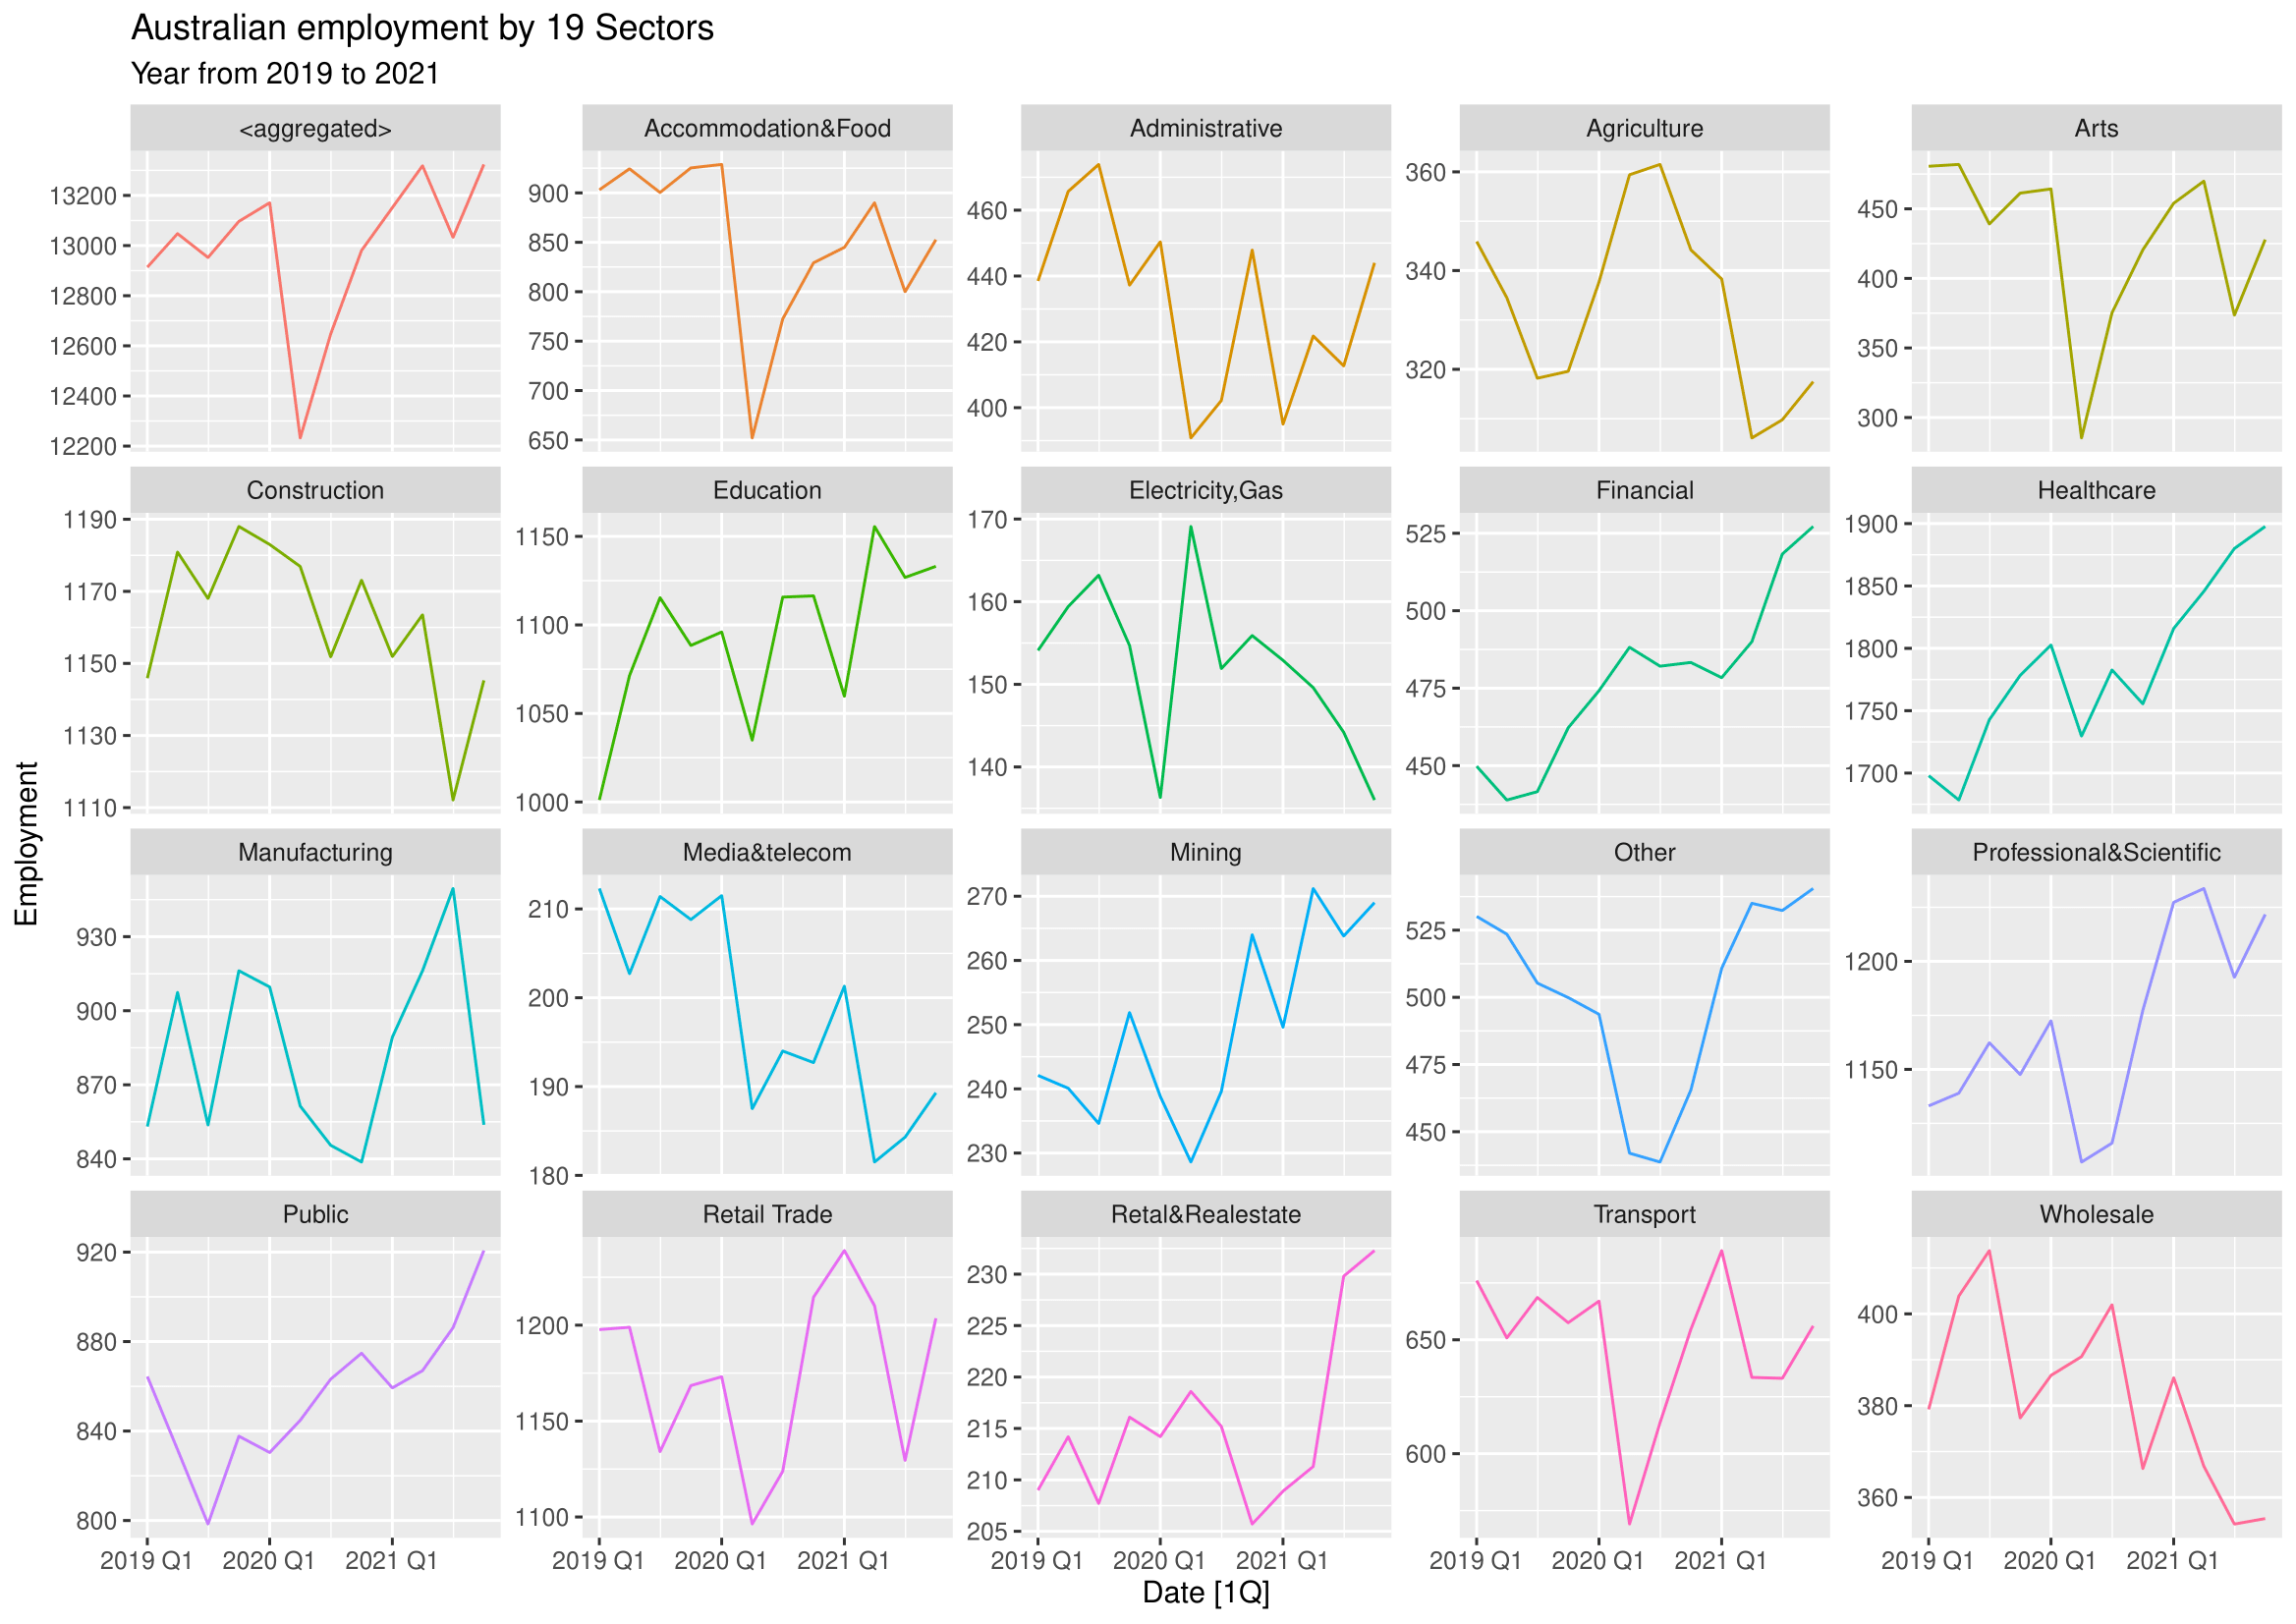
\includegraphics[scale=0.6]{free_19}
\centering
\caption{Employment('000) of 19 sectors in Australia from 2019:Q1 to 2021:Q4}
\label{fig:19}
\end{figure}

\begin{figure}[t]
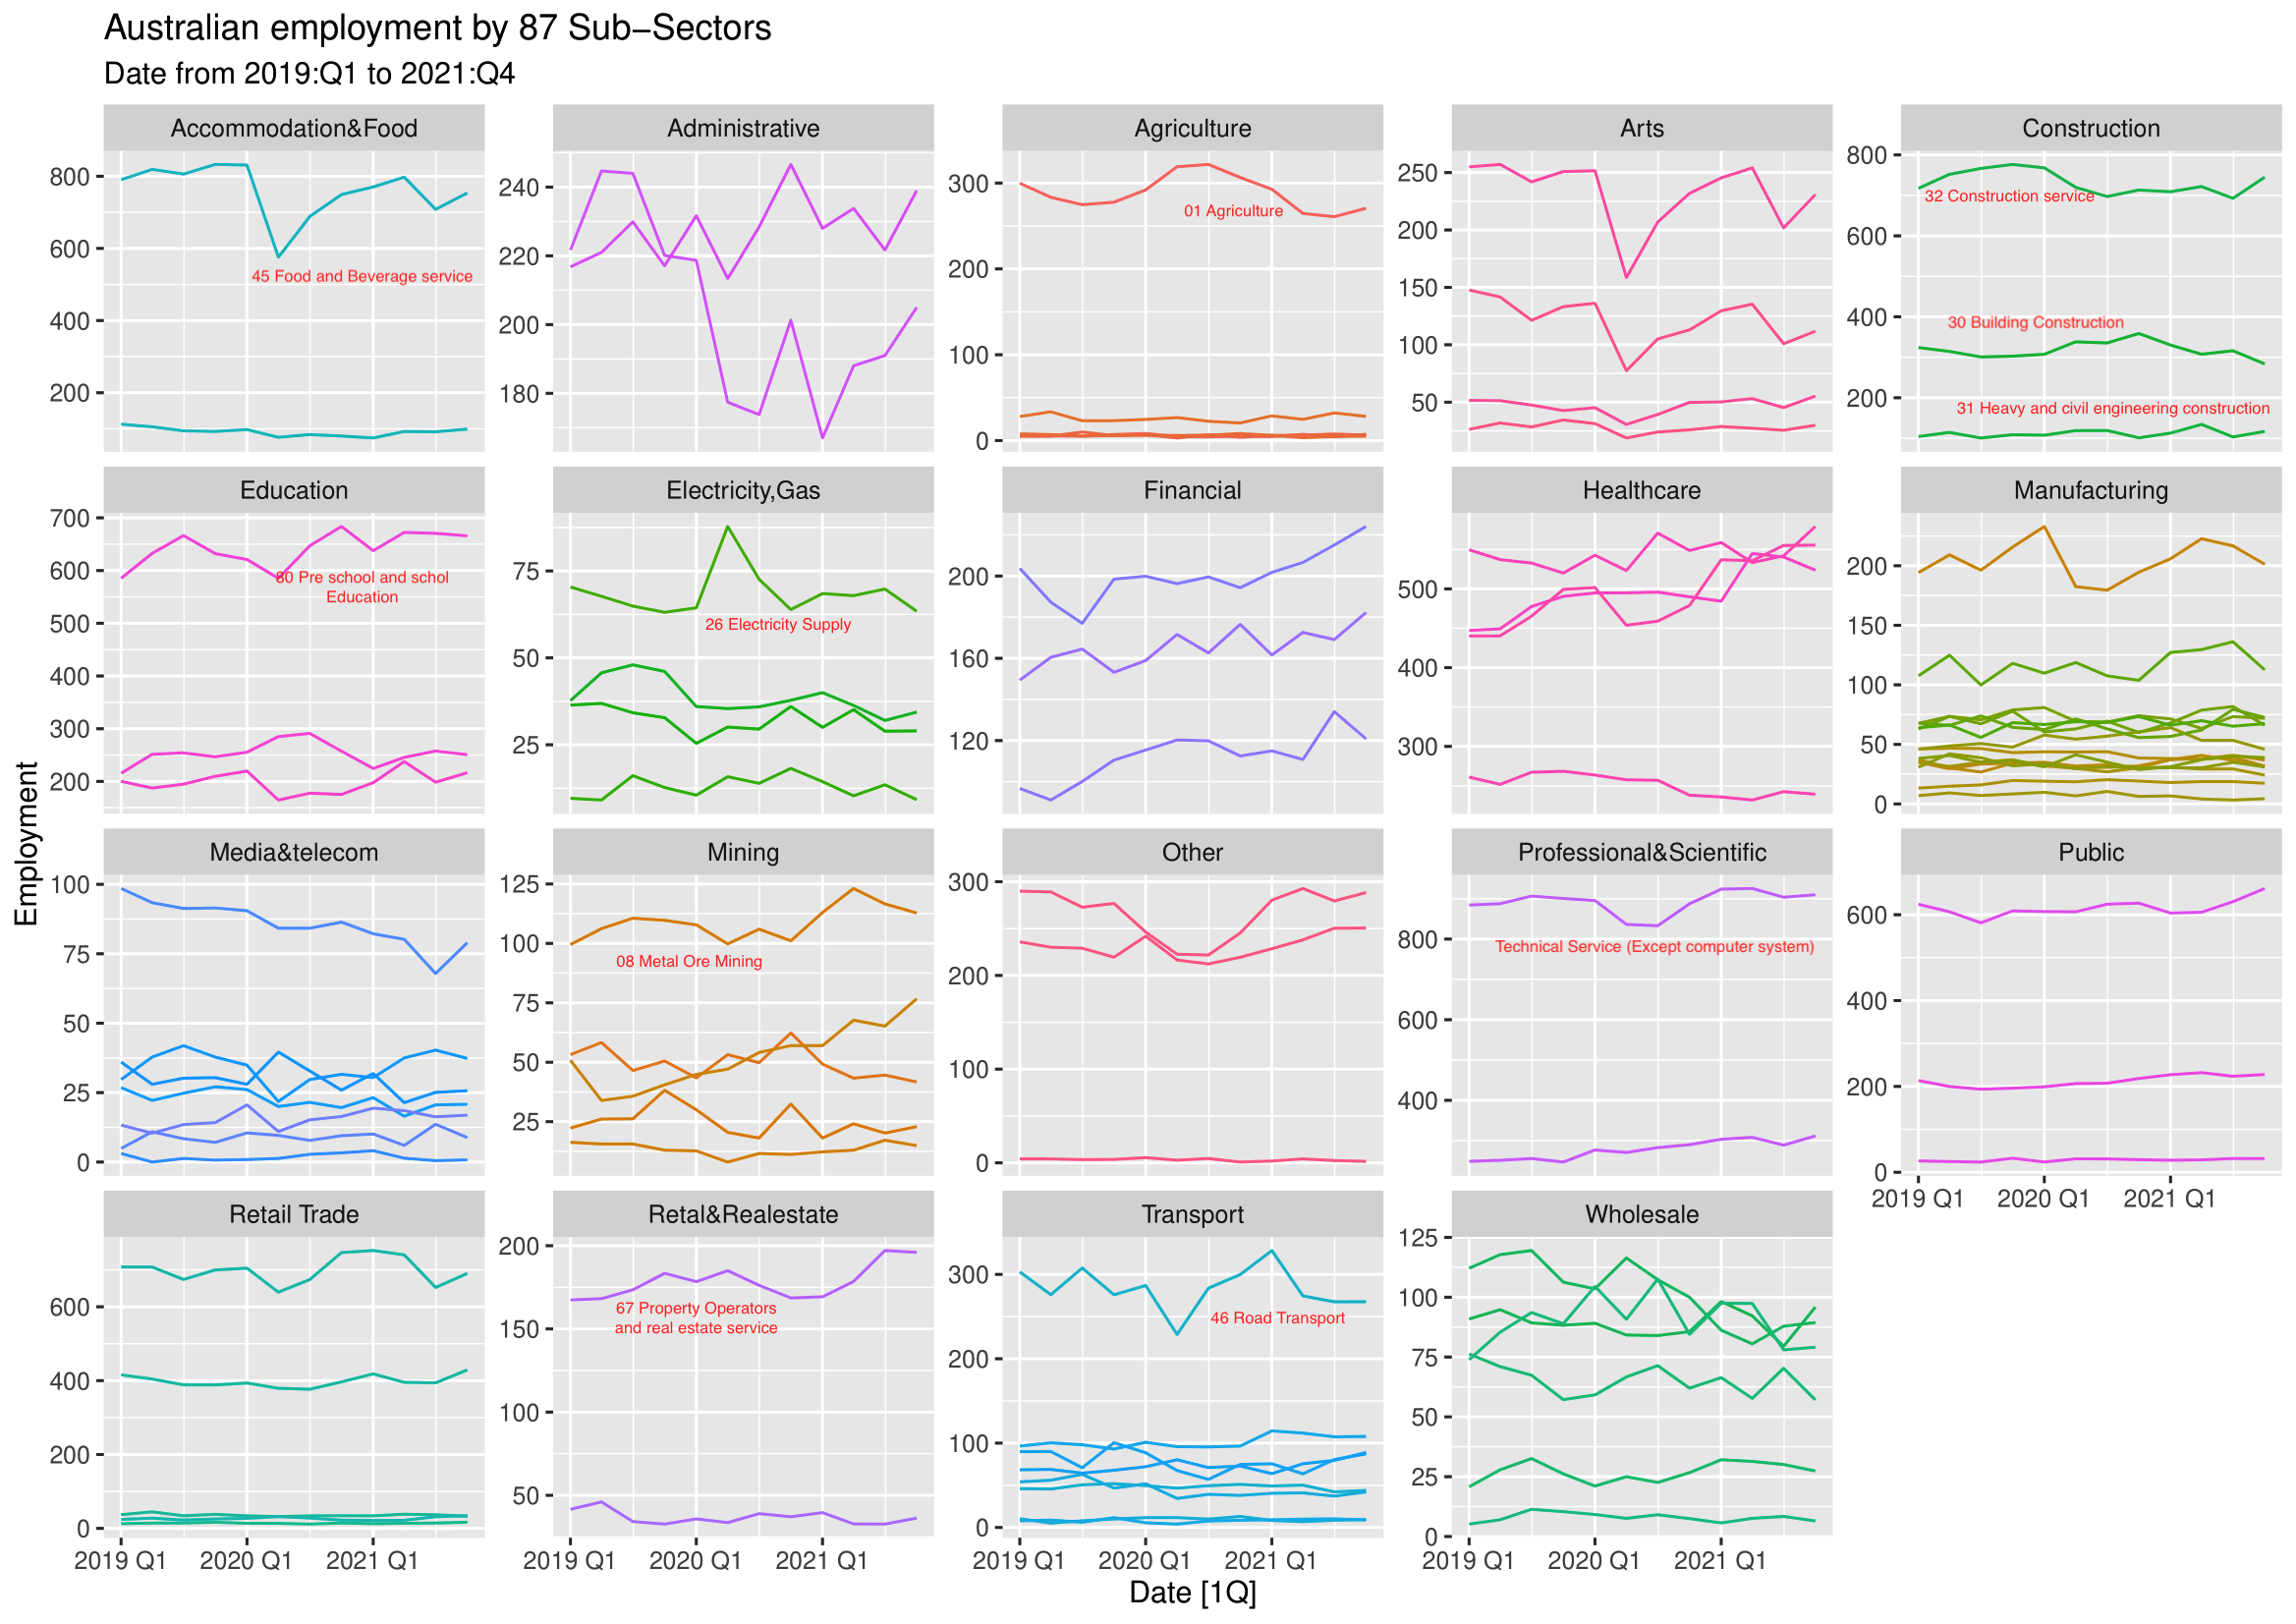
\includegraphics[scale=0.5]{free_87}
\centering
\caption{Employment('000) of 87 two-digit subsectors in Australia from 2019:Q1 to 2021:Q4}
\label{fig:87}
\end{figure}

\begin{figure}[t]
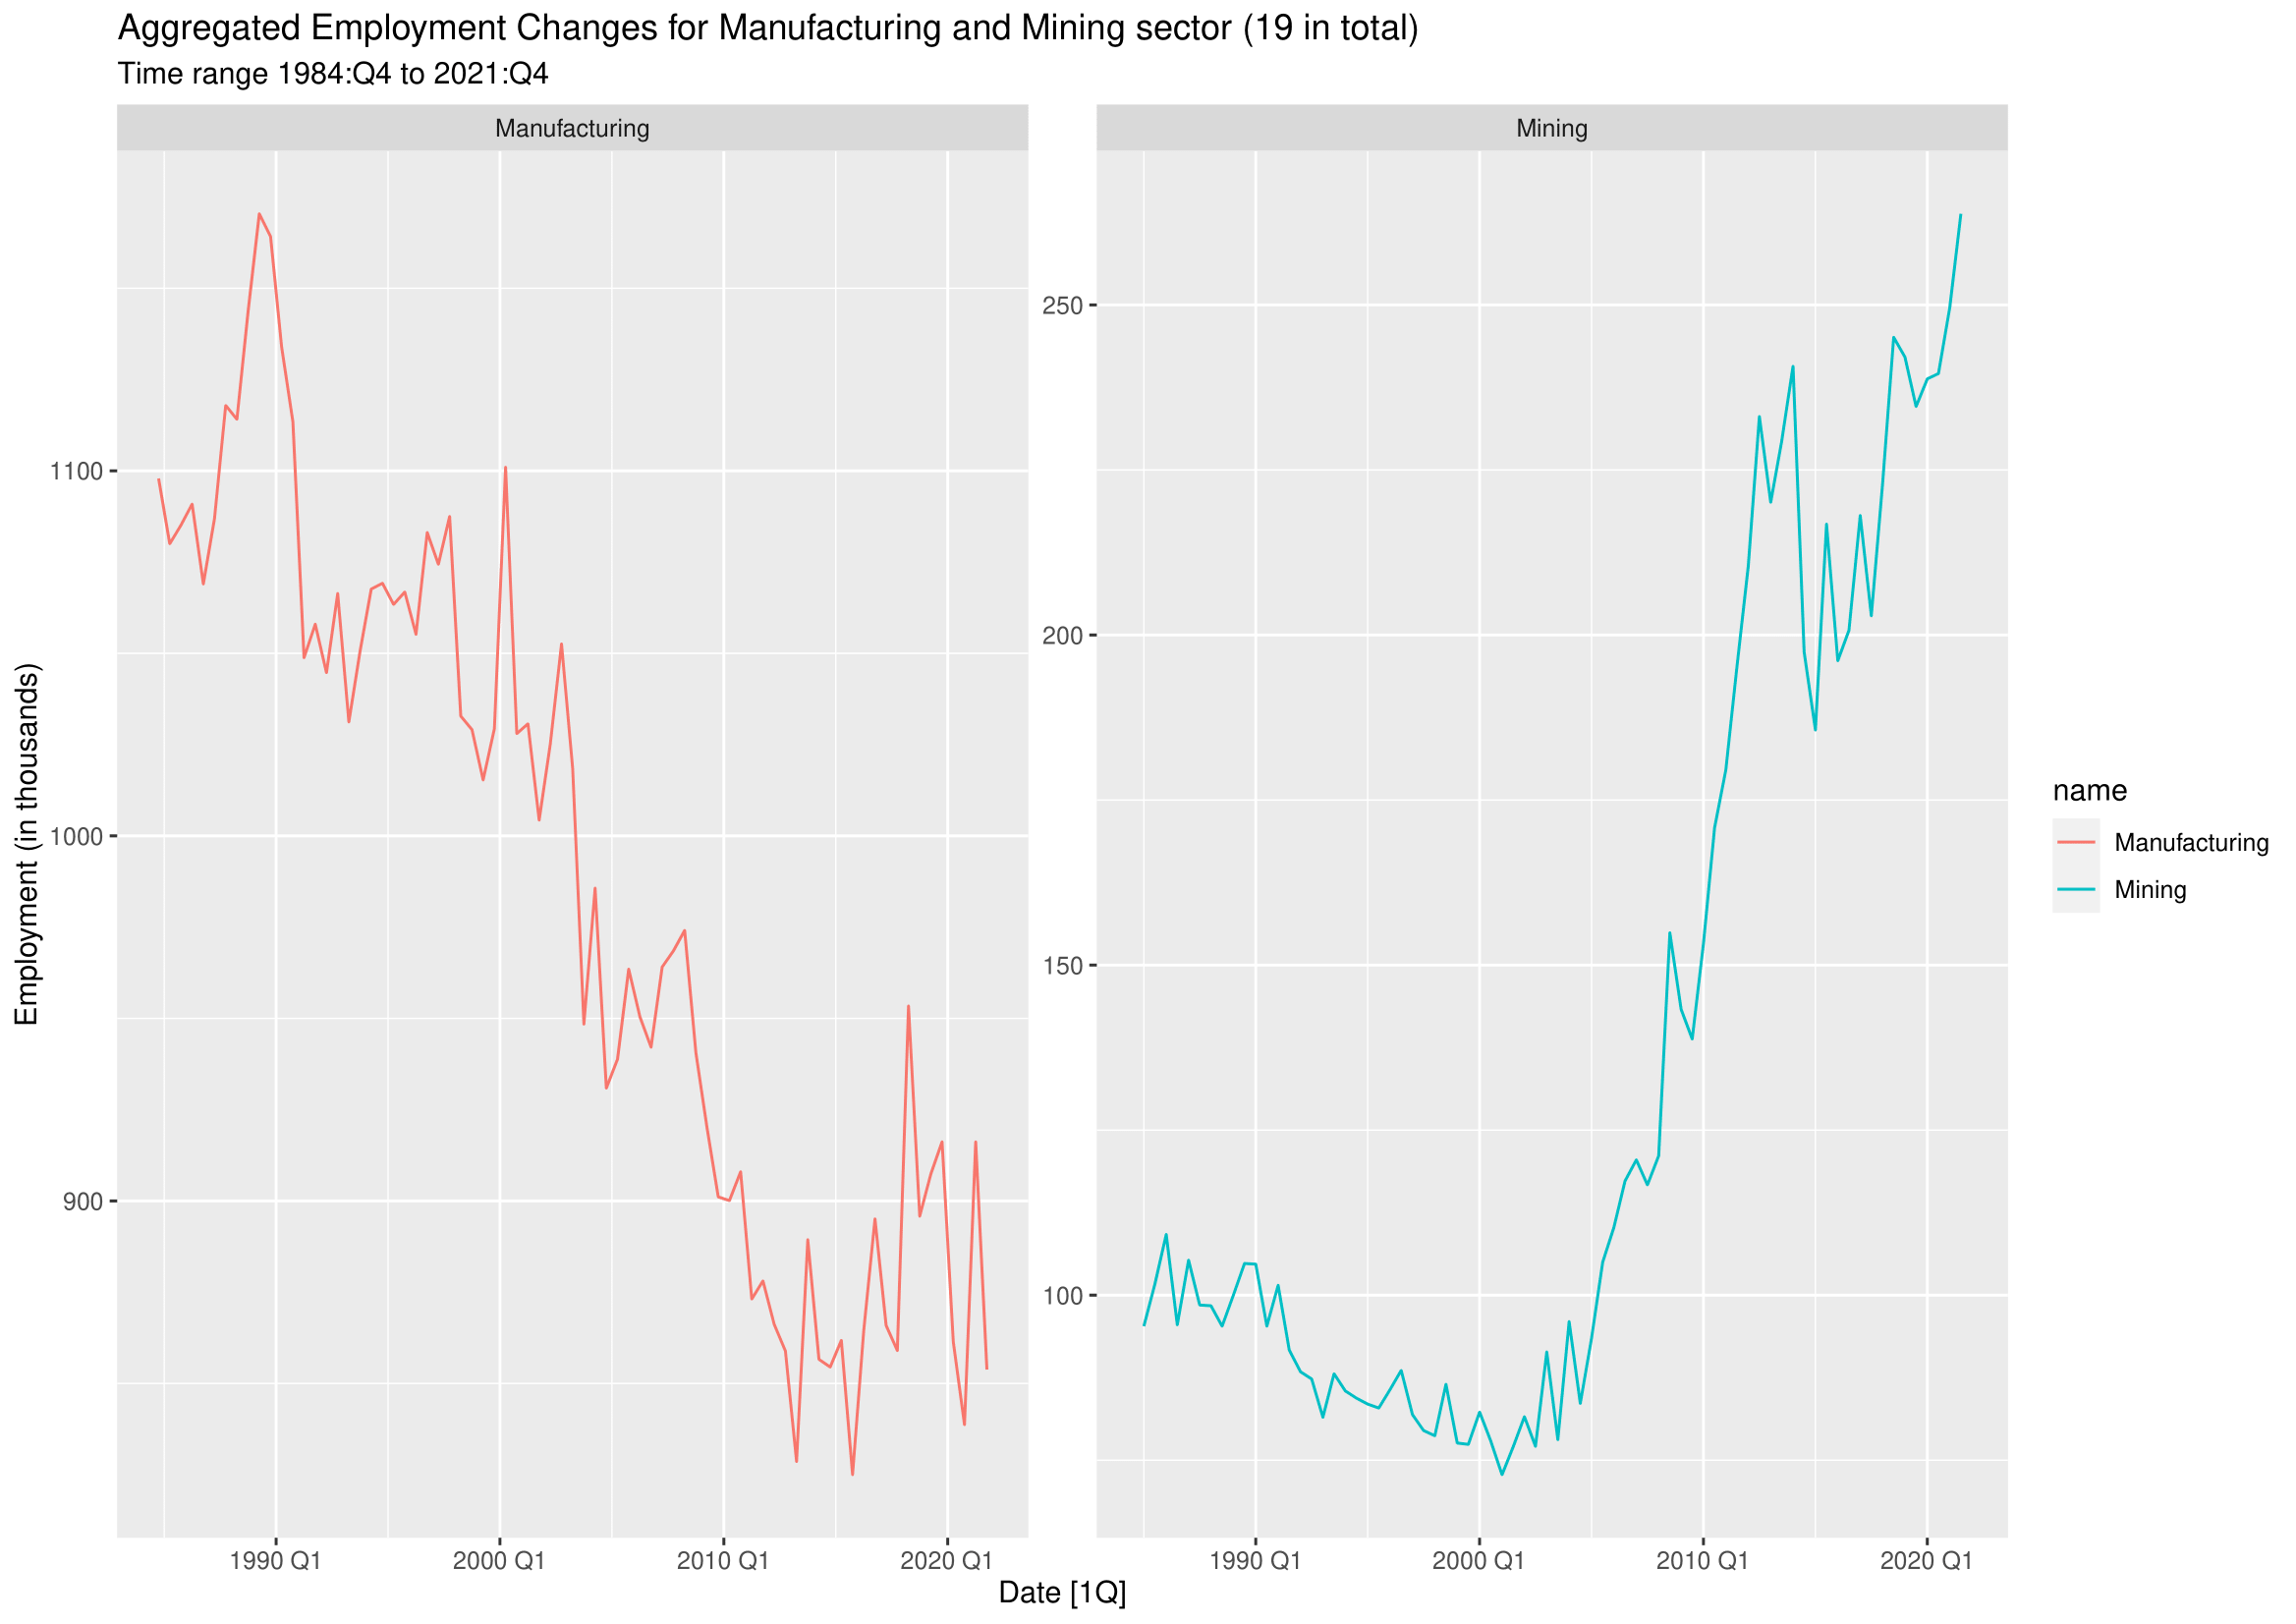
\includegraphics[scale=0.5]{agg_19}
\centering
\caption{Aggregated Employment(in thousands) for Manufacturing and Mining sector in Australia from 1984:Q4 to 2021:Q4}
\label{fig:a19}
\end{figure}

\begin{figure}[t]
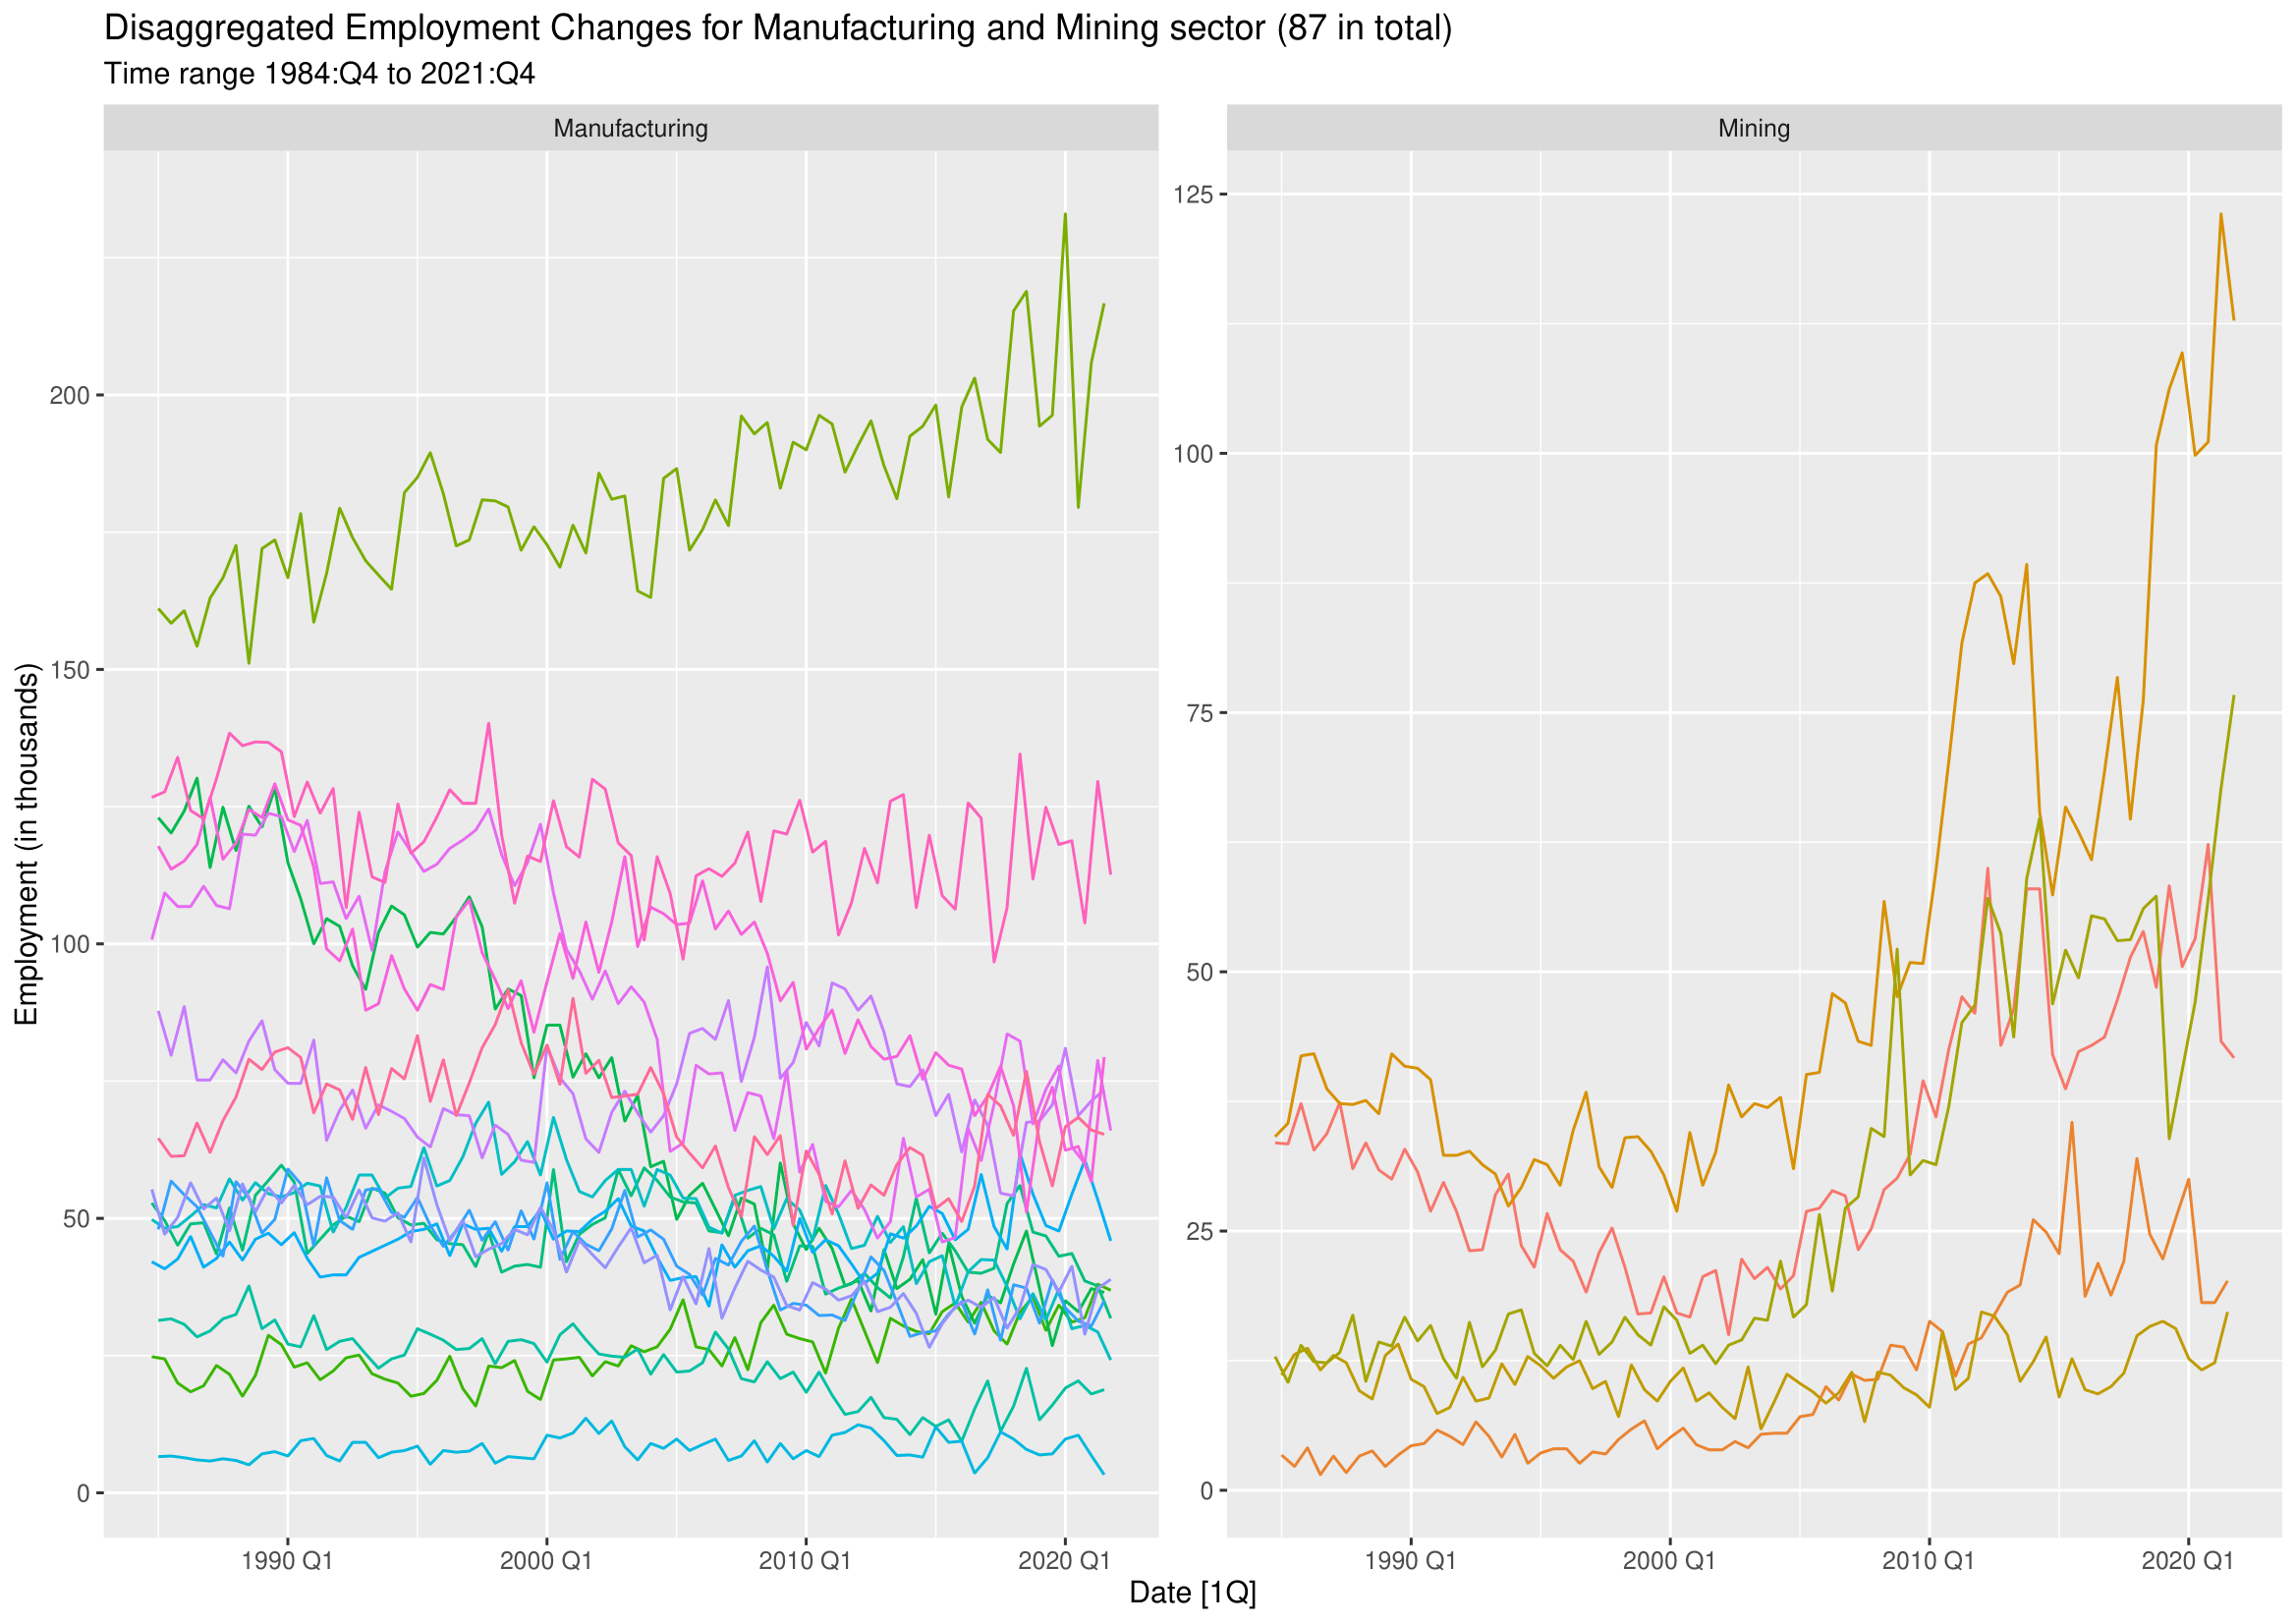
\includegraphics[scale=0.5]{agg_87}
\centering
\caption{Disaaggregate Employment(in thousands) of 87 two-digit subsectors in Manufacturing and Mining sector from 1984:Q4 to 2021:Q4}
\label{fig:a87}
\end{figure}

\begin{figure}[t]
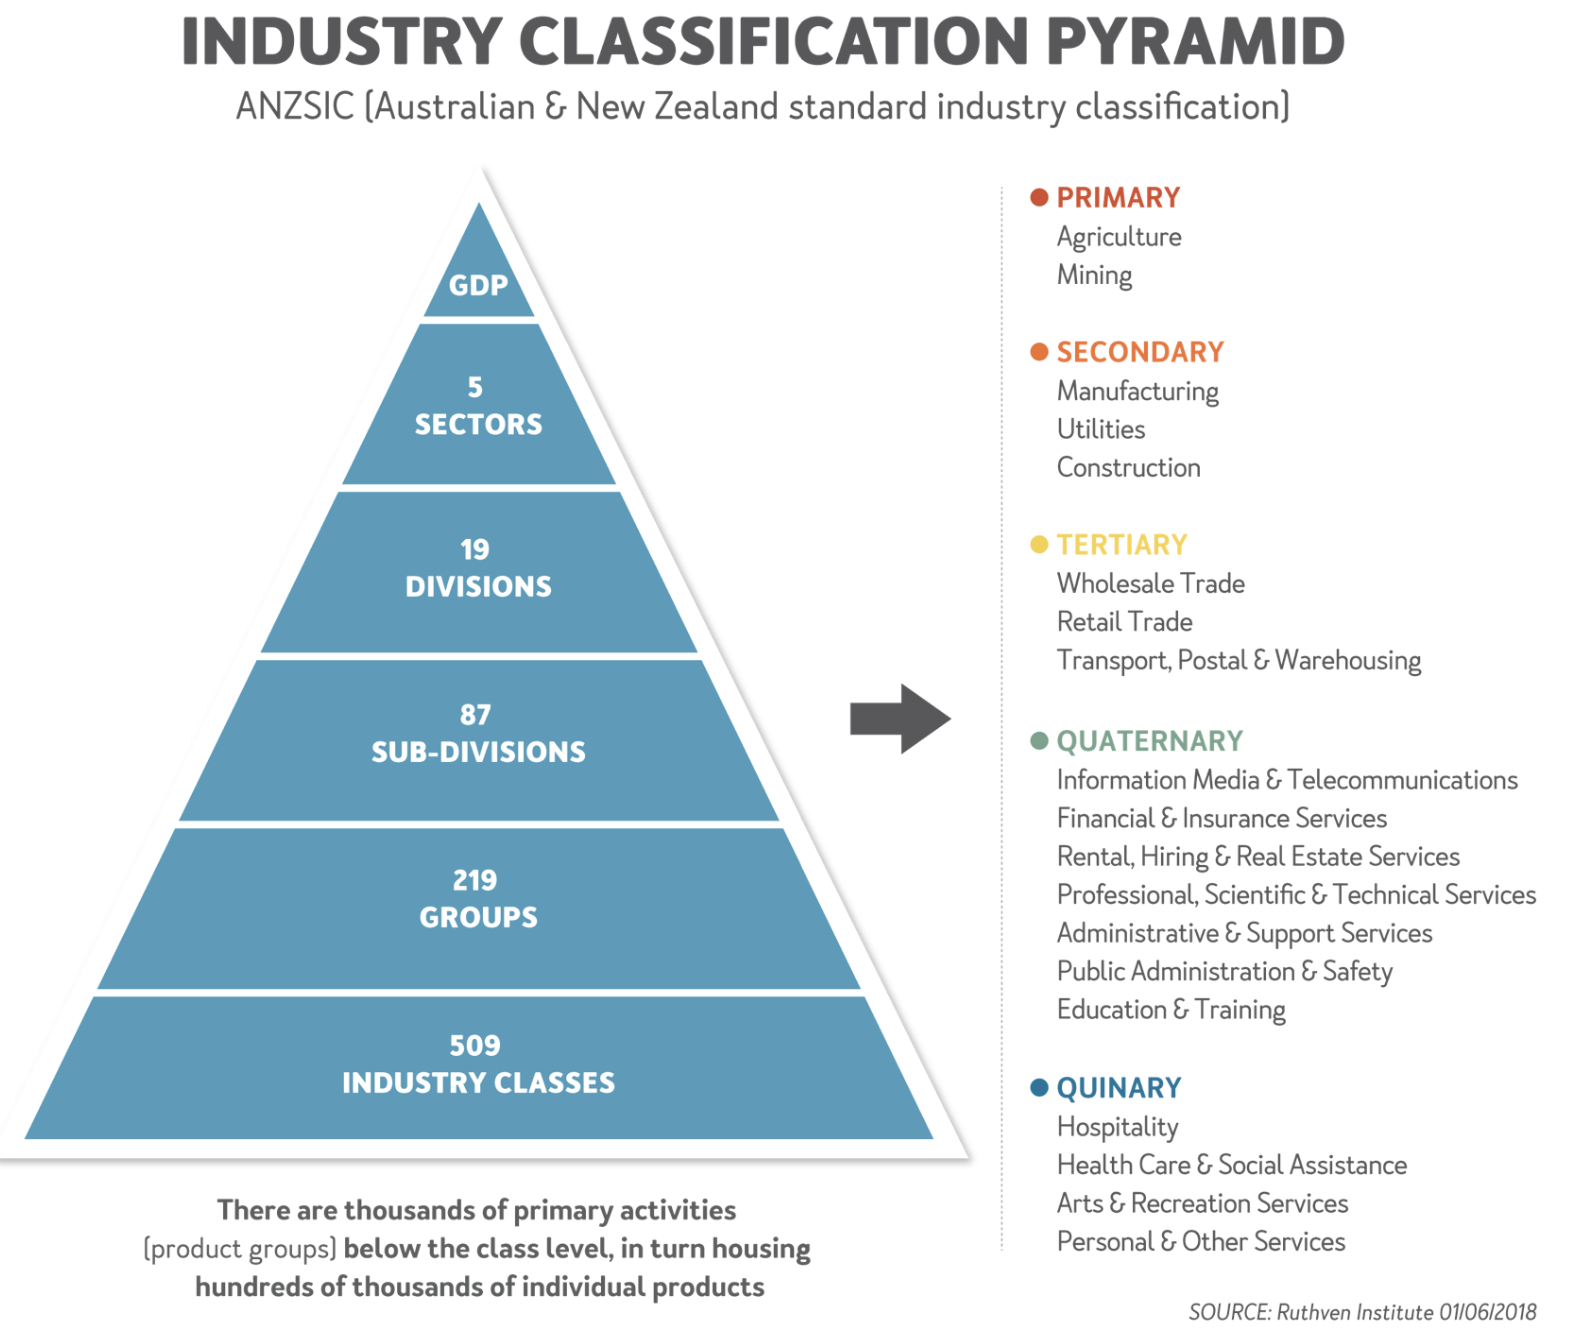
\includegraphics[scale=0.5]{ANZSIC}
\centering
\caption{Australian Industry Pamamid plot by (ANZSIC)}
\label{fig:anzsic}
\end{figure}

\printbibliography[heading=bibintoc]



\end{document}
